
\documentclass{article}

\usepackage{amssymb} %chekmark symbol
\usepackage{graphicx}

\begin{document}

\date{versie 21 maart 2015}
\title{low-level scenario FR-P002}
\maketitle


%%%%%%%%%%%% PUBLICATIE ZOEKEN 
\subsubsection*{PUBLICATIE ZOEKEN IN SKRIBL SYSTEEM EN OP INTERNET}
\vspace{2 mm}

\textbf{ID}: FR-P002
\vspace{2 mm}


\noindent Deze feature bestaat uit twee scenario's: een BASIC search en een ADVANCED search. Bij een basic search wordt er door de gebruiker een enkele string ingegeven, waarna in de database op een bepaald aantal keys wordt gezocht en via GS wordt er een standaard scraping gedaan. Bij een advanced search geeft de gebruiker afzonderlijk titel, jaar, journal e.d. in, waarna in de database bijhorende queries worden uitgevoerd. (Via GS wordt er GEEN advanced search uitgevoerd, dit is enkel mogelijk via dynamische scraping)
\\
\\
zie volgende pagina's

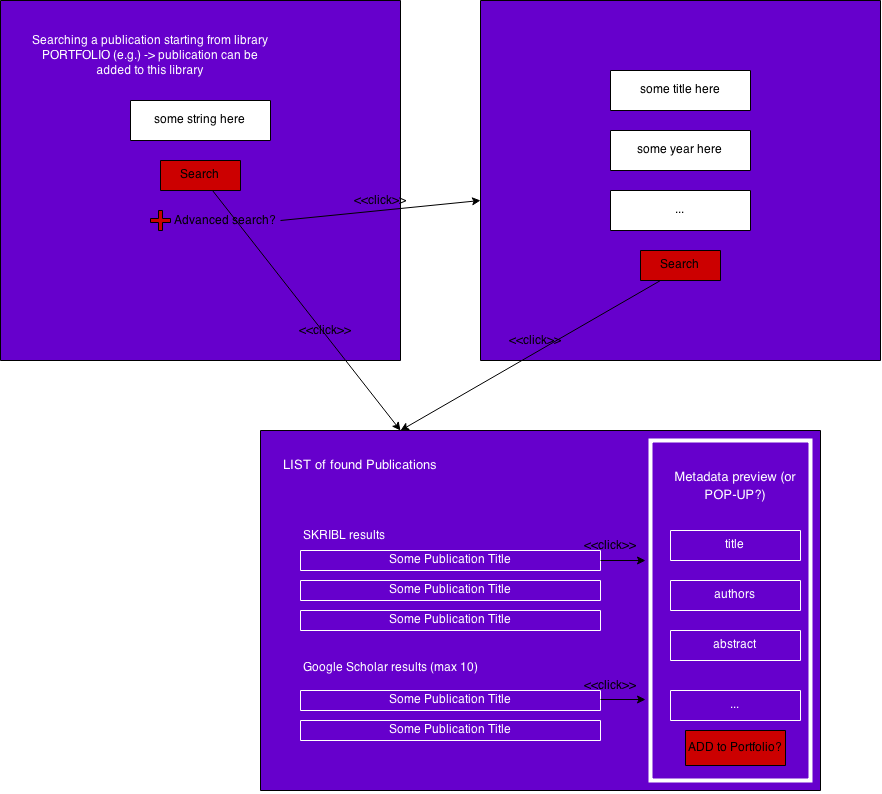
\includegraphics[width=1.3\textwidth]{basic-advanced-search.png}

    


\clearpage

\hrule
\vspace{2 mm}
\noindent \textbf{Scenario}:
\begin{description}
\item CLIENT : G wil publicatie zoeken om eventueel toe te voegen aan bibliotheek, e.g. gebruiker is in 'PORTFOLIO' en klikt op publicatie zoeken  
	\begin{description}
	\item \checkmark validatie gegeven input (afhankelijk van advanced of basic search)
	\item $\rightarrow$ GET /publications 
	\end{description}
	
\item SERVER : 
	\begin{description}
	\item \checkmark validatie
	\item $\leftarrow$ gevonden resultaten: JSON met
		\begin{description}
		\item resultaten van google scholar: max 10 JSON metadata (\emph{overleg met front})
		\item resultaten van skribl: publicatie ID + titel; via ID kan later metadata opgevraagd worden aan server om deze weer te geven. Voor een basic search zijn deze resultaten van een (partial) match in de database met:
			\begin{description}
			\item auteur
			\item titel
			\item journal of proceeding
			\item keywords
			\item (universiteit)
			\end{description}
		\end{description}
	\end{description}
	
\item CLIENT :  G ziet een lijst van resultaten (titel van de publicaties) en kan een publicatie aanklikken om meer informatie te zien 
	\begin{description}
	\item $\rightarrow$ indien SKRIBL resultaat: GET /publications/<pub-id>, voor GS resultaat metadata reeds aanwezig na vorige request (\emph{overleg met front})
	\item pop-up of side menu preview van metadata 
	\end{description}
	
\item CLIENT :  G wil publicatie toevoegen aan bibliotheek
	\begin{description}
	\item !!!!!   indien GS resultaat: 
		\begin{description}
		\item metadata moet manueel aangevuld worden op zelfde manier als bij publicatie uploaden met bijhorende requests en validaties, checken of publicatie al in Sribl systeem zit, checken of auteurs al in systeem zitten ed. 
		\item dus eerste een PUT /publications met de gevonden URL; server zal de publicatie proberen downloaden 
		\item daarna POST /publications/<pub-id> zoals in FR-P001
		\end{description}
	\item SKRIBL resultaat $\rightarrow$ PUT /user/<username>/library/<libraryname>/<publication-id>
	\end{description}
			
\item CLIENT :  message: publicatie toegevoegd aan huidige bibliotheek.

 \end{description}
 
\end{document}





